% Copyright (C)  2015  Philipp Hacker.
% Permission is granted to copy, distribute and/or modify this document
% under the terms of the GNU Free Documentation License, Version 1.3
% or any later version published by the Free Software Foundation;
% with no Invariant Sections, no Front-Cover Texts, and no Back-Cover Texts.
% The lincense itself can be found at <https://www.gnu.org/licenses/fdl-1.3>.

\documentclass[numbers=noenddot,a4paper]{scrartcl}

\usepackage[greek,ngerman]{babel}
\usepackage[T1]{fontenc}
\usepackage[utf8]{inputenc}
\usepackage{fullpage}
\usepackage{scrpage2}
\usepackage{libertine}
\usepackage{ziffer}
\usepackage{graphicx}
\usepackage{units}
\usepackage[infoshow]{tabularx}
\usepackage[all]{xy}
\usepackage{amsmath}
\usepackage{amssymb}
\usepackage{wrapfig}
\usepackage{upgreek}
\usepackage{esint}
\usepackage{float}
\usepackage[font=small,labelfont=bf]{caption}
\usepackage{subcaption}
\usepackage{lscape}
\usepackage[backref=page]{hyperref}
\usepackage{csquotes}
\usepackage[printonlyused,withpage,footnote]{acronym}

\renewcommand{\thefigure}{Abb. \arabic{figure}}
\renewcommand{\bflabel}[1]{\normalfont{\normalsize{#1}}\hfill}

%\captionsetup[wrapfigure]{name=}
\captionsetup[figure]{name=}

\newcommand{\nummat}[1]{\left[\text{#1}\right]}
\newcommand{\num}[1]{$\left[\text{#1}\right]$}
\newcommand{\degree}{^\circ}
\newcommand{\diff}{\textnormal{d}}
\newcommand{\tenpo}[1]{ 10^{#1}}
\newcommand{\greek}[1]{\greektext#1\latintext}
\newcommand{\ix}[1]{_\text{#1}}
\newcommand{\imag}{\mathbf{i}}
\newcommand{\tilt}[1]{\textit{#1}}
\newcommand{\grad}[1]{\textit{grad}\left(#1\right)}
\newcommand{\divergenz}[1]{\textit{div}\left(#1\right)}
\newcommand{\euler}{\mathnormal{e}}
\newcommand{\fett}[1]{\textbf{#1}}

\title{Bachelor-Arbeit zum Thema \enquote{Modenanregung in \tilt{Yukawa}-Bällen}} %TODO Name
\author{Philipp Hacker} %TODO Author
\date{\today}

\setcounter{section}{-1}


\begin{document}
	
	\maketitle
	
	\begin{center}
		
		Institut für Physik\\
		mathematisch-naturwissenschaftliche Fakultät\\
		Universität Greifswald
		
	\end{center}
	 
	\vspace{0.5cm}
	
	\begin{figure}[H]
			\centering
			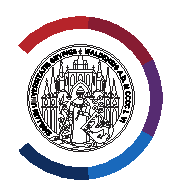
\includegraphics[width=0.35\textwidth]{/home/pha/git/bachelor_arbeit-philipp_hacker/figs/unilogo_NEU_schwarz.eps}
	\end{figure}
	
	\vspace{0.5cm}
	
	\begin{center}
			
			\hspace{-0.55cm} Erst-Gutachter: Prof. Dr. André Melzer \\ \vspace{0.25cm} %TODO Name Erst-Gutachter
			
			Zweit-Gutachter: Prof. Dr. Lutz Schweikhard \\ \vspace{0.25cm} %TODO Name Zweit-Gutachter
			
			Bearbeitungszeitraum: 01.03.2015 bis 12.07.2015 \\ \vspace{0.25cm} %TODO Bearbeitungszeitraum
		
%		\begin{table}[h]
%			\centering
%			Note (Erst-Gutachter): %TODO Gute Note erhalten :)
%			\begin{tabularx}{1.5cm}{|X|}
%				\hline \\ \\
%				\hline
%			\end{tabularx}
%			
%			\centering
%			\hspace{-0.42cm} Note (Zweit-Gutachter): %TODO Gute Note erhalten :)
%			\begin{tabularx}{1.5cm}{|X|}
%				\hline \\ \\
%				\hline
%			\end{tabularx}
%			
%		\end{table}

	\end{center}
	
	\thispagestyle{empty}
	
	\newpage
	
	\tableofcontents
	
	\newpage
	
	\section{Motivation}\label{sec:einleitung}
	
		Test der Literaturbibliothek \cite{Thomas94}
		
	\newpage
	
	\section{Physikalische Grundlagen}\label{sec:physg}
	
		\subsection{Aufladung von Staubpartikeln in einem Plasma}\label{subsec:ströme}
	
		\subsection{Staub-Dynamik im Plasma}\label{subsec:dynamik}
		
				In einem Plasma wirken viele, u.U. nicht-triviale Kräfte auf den eingefangenen Staub. Im Folgenden werden die wichtigsten Einflüsse auf die Dynamik komplexer Plasmen vorgestellt und beschrieben.\\
				
				\subsubsection{Gravitation und elektrische Feldstärke}\label{subsub:grav}
				
				Betrachtet man ein Experiment, welches am Erdboden in Nähe der Meereshöhe durchgeführt wird, so muss offensichtlich die vollständige Gravitationskraft berücksichtigt werden. Dies gilt bspw. nicht für Versuche unter Mikrogravitation während Parabelflügen oder in Höhen von mehr als $\unit[80]{km}$.
				
					\begin{align}
						F\ix{G}=m\ix{S} g=\frac{4}{3}\pi a^3 \rho\ix{S} g
					\end{align}
				
				($m\ix{S}$ - Masse der Staubteilchen; $a$ - Partikelradius; $\rho\ix{S}$ - Massendichte des Staubes; $g$ - \mbox{Erdbeschleunigung})\\
				Natürlich wirkt auf die, durch das ionisierte Gas elektrisch geladenen Partikel eine elektrische Kraft $F\ix{E}$, welche aus dem äußeren Feld $E$ der Plasma-Elektroden folgt. Eine elektrische Wechselwirkung mit dem Plasma tritt aufgrund der Quasineutralität nicht auf: innerhalb einer \tilt{Debye-Kugel} sind die Veränderung zu schnell, als dass das träge Staubteilchen diesen folgen könnte. 
				
					\begin{align}
					F\ix{E}=Q\ix{S} E=4 \pi \epsilon\ix{0} a \Phi\ix{fl} E
					\end{align}
		
				($Q\ix{S}$ - Staubladung; $\Phi\ix{fl}$ - \tilt{floating}-Potential)\\
				Diese beiden Kräfte heben sich gerade in der Randschicht einer sog. Radiofrequenz-Entladung (\tilt{rf discharge}) auf, da sie für eine oben liegende Kathode antiparallel stehen. Zu beachten ist hierbei der stark unterschiedliche Einfluss des Teilchenradius - $\propto a^3$ und $\propto a$.\\
								
				\subsubsection{Abschirmung und Polarisationskräfte}\label{subsub:abschirm}
				
				Die große negative Aufladung der Staubteilchen sorgt über die Coulomb-Wechselwirkung mit den auf das Partikel zuströmenden Ionen dafür, das sich eine Konzentration derer lokal stark ändert. Es entsteht eine Wolke aus langsamen Ionen die quasi in der näheren Umgebung um das Teilchen verbleiben, jedoch nicht mit diesem interagiert und es nach außen hin vor dem Einfall schnellerer pos. Ladungen abschirmen. Somit gibt es keine direkte Rückwirkung der Wolke auf das Partikel, sofern dessen sphärische Symmetrie gegeben ist. Gilt dies nicht, so entsteht ein Multipol- bzw. Dipolmoment $\vec{p}$, welches danach strebt, sich in Richtung des Feldes $\vec{E}$ auszurichten. Damit wirkt eine Kraft $F\ix{Dip}$ (für ein Dipolmoment) auf das Staubteilchen zurück, welche mit dem Gradienten der Richtungsdifferenz zwischen $\vec{p}$ und $\vec{E}$ geht.

					\begin{align}
						\centering
						\vec{F}\ix{Dip}&=\vec{\nabla}\left(\vec{p}\vec{E}\right)\\
						&{\overset{\vec{p}\,||\vec{E}}{=}}\grad{pE} \nonumber
					\end{align}
					
				Das besagte Dipolmoment entsteht u.a. durch die diversen, gerichteten Ladungsprozesse in dem Plasma. Ein Partikel, welches in der Randschicht eingefangen und von einer Ionenwolke umgeben wird, 'sieht' unterschiedliche \tilt{Debye}-Längen über und unter sich aufgrund der lokalen Feldrichtung und der stark vom Mittelwert abweichenden Ionen- und Elektronendichten. Somit ändert sich offensichtlich die Plasmadichte innerhalb des Volumens einer Kugel mit dem, nun ortsabhängigen Radius $\lambda\ix{D}\left(\vec{r}\right)$. Insgesamt folgt daraus eine neue Bestimmungsgleichung für das Potential und damit auch eine neue Kraft $F\ix{E}$.
				
					\begin{align}
						\Delta \Phi\left(\vec{r}\right)-\frac{\Phi\left(\vec{r}\right)}{\lambda\ix{D}^2\left(\vec{r}\right)}=\frac{Q\ix{s}}{\epsilon\ix{0}}\delta\left(\vec{r}\right) \\
						F\ix{E}=\underbrace{Q\ix{S}E}_{\text{(I)}}-\underbrace{\frac{Q\ix{S}^2}{8\pi\epsilon\ix{0}}\frac{\nabla\lambda\ix{D}\left(\vec{r}\right)}{\lambda\ix{D}^2}}_{\text{(II)}}
					\end{align}
				
				Hierbei stellt (I) die normale Komponente dar und (II) ist zusätzliche Kraft durch die Deformation der Ionenwolke in Richtung kleinerer \tilt{Debye}-Längen $\lambda\ix{D}\left(\vec{r}\right)$. Die Kraft $F\ix{E}$ kann also dadurch größer oder kleiner werden. Hinzu kommt, dass der veränderte Parameter $\lambda\ix{D}$ von der Driftgeschwindigkeit $u\ix{I}$ abhängt, welche die Ionenwolke maßgeblich beeinflusst. Ist jedoch $u\ix{I}<v\ix{th,I}$ so kann man annehmen, dass die Ionenwolke besteht und $\lambda\ix{D}\left(\vec{r}\right)\approx\lambda\ix{D,I}$ gilt.\\
				Sind die Ionen jedoch schneller, womit $u\ix{I}>>v\ix{th,I}$ wird, so können sie nicht mehr vom Feld des Partikels 'gefangen' werden und damit die Ionenwolke bilden. So gilt folglich $\lambda\ix{D}\left(\vec{r}\right)\approx\lambda\ix{D,e}$.\\
				Insgesamt ist der Einfluss der Polarisation vernachlässigbar klein, solange die Teilchen eine Größe von einigen hundert $\unit{\mu m}$ nicht übersteigen.

			\subsubsection{Ionen-/Neutralgasreibung}\label{subsub:reibung}

				Aufgrund der hohen negativen Ladung des Staubteilchens und der daraus resultierenden elektrostatischen Wechselwirkung existiert ein, relativ auf das Partikel zufließender, Ionenstrom. Weiterhin bewegen sich mit ihrer thermischen Geschwindigkeit die Neutralgasatome durch das Plasma und stoßen mit anderen Teilchen. Die Zahl der Stöße $\diff N$ einer Spezies mit einem Target mit dem Streuparameter $\sigma$ im Zeitintervall $\diff t$ ist somit über deren relative Geschwindigkeit $v\ix{rel}$ zu diesem in $\diff N=n\sigma v\ix{rel}\diff t$ gegeben. Hierbei kennzeichnet $n$ die Stromdichte der strömenden Teilchen. Aus diesem Strom folgt ein gewisser Impulsübertrag $\Delta p$ auf das Target. Hieraus lässt sich eine Kraft $F\ix{drag}$ ziehen, die einer Reibung bzw. einer Impulsaufnahme entspricht.
				
					\begin{align}
						F\ix{drag}=\frac{\diff N \Delta p}{\diff t}=\Delta p n \sigma v\ix{rel}
					\end{align}
					
				Man spricht hierbei auch von \tilt{ambipolarer Diffusion}, da die Ionenströme und damit auch die Ionenreibung zu beiden Polen führen. Man kann diese aus 2 Teilen aufbauen: direkte Kollisionen mit den Ionen $F\ix{dir}$ und deren Coulomb-Streuung an den Feldern der neg. geladenen Staubpartikel. Im folgenden soll das sog. \tilt{Barnes-Modell} eingeführt werden, welches die besagte Ionenreibung beschreibt.
				
				\paragraph{Ionenreibung: \tilt{Barnes-Modell}}
				
				Für die Bestimmung von $F\ix{dir}$ wird angenommen, dass nur die Ionen, welche für eine Ladungsänderung der Partikel sorgen, auch diese direkt treffen. Im Rückblick auf die Bestimmung der Ionenströme in \ref{subsec:ströme} wird die Kraft durch Kollisionen zu
				
					\begin{align}
						F\ix{dir}=\pi a^2m\ix{I}\tilde{v}n\ix{I}u\ix{I}\left(1-\frac{2e\Phi\ix{Fl}}{m\ix{I}\tilde{v}^2}\right)\,\,.
					\end{align}
					
				($n\ix{I}$ - Ionenkonzentration; $u\ix{I}$ - Ionen-Driftgeschwindigkeit; $m\ix{I}$ - Ionenmasse)\\
				Das Produkt aus Masse und mittlerer Geschwindigkeit der Ionen $m\ix{I}\tilde{v}=m\ix{I}\sqrt{u\ix{I}^2+v\ix{Th,I}^2}$ entspricht dem Impulsübertrag.\\
				Für die Coulomb-Streuung müssen alle diejenigen Ionen miteinbezogen werden, welche mit dem Feld des Staubes 'stoßen'. Hierfür wird der Streuquerschnitt $\tilde{\sigma}$ der Ionen-Elektronen-Wechselwirkung auf den aktuellen Fall angepasst.
				
					\begin{align}
						\tilde{\sigma}=4\pi b_{\frac{\pi}{2}}^2\ln\left(\Lambda\right)=&\,4\pi b_{\frac{\pi}{2}}^2\ln\left(\frac{\lambda\ix{D}}{b_{\frac{\pi}{2}}}\right) \\
						b_{\frac{\pi}{2}}=&\,\frac{e^2}{4\pi\epsilon\ix{0}m\ix{I}v^2} \nonumber
					\end{align}
					
				Der Stoßparameter $b_{\frac{\pi}{2}}$ beschreibt eine Ablenkung um $\unit[90]{\degree}$. Für die Ionenreibung müssen weitere Bedingungen mit eingebunden werden: die Coulomb-Streuung außerhalb der Ionenwolke ist irrelevant, die Staubpartikel haben eine endliche Ausdehnung und damit existiert ein minimaler Stoßparameter $b\ix{k}$. Damit wird das gesuchte $\sigma$ zu
				
					\begin{align}
						\sigma=\int_{b\ix{k}}^{\lambda\ix{D}}\tilde{\sigma}\diff\left(\frac{\lambda\ix{D}}{b_{\frac{\pi}{2}}}\right)=&\,4\pi b_{\frac{\pi}{2}}^2\ln\left(\frac{\lambda\ix{D}^2+b_{\frac{\pi}{2}}^2}{b\ix{k}^2+b_{\frac{\pi}{2}}^2}\right)^{1/2} \nonumber \\
						\overset{*}{=}&\,\frac{2\pi a^2 e^2\Phi\ix{Fl}^2}{m\ix{I}\tilde{v}^3}n\ix{I}u\ix{I}\ln\left(\frac{\lambda\ix{D}^2+b_{\frac{\pi}{2}}^2}{b\ix{k}^2+b_{\frac{\pi}{2}}^2}\right)^{1/2} \, \, .
					\end{align}

	\newpage
	
	\section{Durchführung}\label{sec:durch}
	
	\newpage
	
	\section{Auswertung}\label{sec:auswert}
	
	\newpage
	
	\section{Literatur}\label{sec:lit}
	
		\bibliography{all_melzer.bib}
		\bibliographystyle{unsrt}
	
	\newpage
	
	\section{Anhang}\label{sec:anhang}
	
%		\subsection{Abkürzungsverzeichnis}\label{subsec:abkurz}
%		
%			\begin{acronym}
%				
%			\end{acronym}
	
\end{document}